\documentclass{article}[18pt]
\ProvidesPackage{format}
%Page setup
\usepackage[utf8]{inputenc}
\usepackage[margin=0.7in]{geometry}
\usepackage{parselines} 
\usepackage[english]{babel}
\usepackage{fancyhdr}
\usepackage{titlesec}
\hyphenpenalty=10000

\pagestyle{fancy}
\fancyhf{}
\rhead{Sam Robbins}
\rfoot{Page \thepage}

%Characters
\usepackage{amsmath}
\usepackage{amssymb}
\usepackage{gensymb}
\newcommand{\R}{\mathbb{R}}

%Diagrams
\usepackage{pgfplots}
\usepackage{graphicx}
\usepackage{tabularx}
\usepackage{relsize}
\pgfplotsset{width=10cm,compat=1.9}
\usepackage{float}

%Length Setting
\titlespacing\section{0pt}{14pt plus 4pt minus 2pt}{0pt plus 2pt minus 2pt}
\newlength\tindent
\setlength{\tindent}{\parindent}
\setlength{\parindent}{0pt}
\renewcommand{\indent}{\hspace*{\tindent}}

%Programming Font
\usepackage{courier}
\usepackage{listings}
\usepackage{pxfonts}

%Lists
\usepackage{enumerate}
\usepackage{enumitem}

% Networks Macro
\usepackage{tikz}


% Commands for files converted using pandoc
\providecommand{\tightlist}{%
	\setlength{\itemsep}{0pt}\setlength{\parskip}{0pt}}
\usepackage{hyperref}

% Get nice commands for floor and ceil
\usepackage{mathtools}
\DeclarePairedDelimiter{\ceil}{\lceil}{\rceil}
\DeclarePairedDelimiter{\floor}{\lfloor}{\rfloor}

% Allow itemize to go up to 20 levels deep (just change the number if you need more you madman)
\usepackage{enumitem}
\setlistdepth{20}
\renewlist{itemize}{itemize}{20}

% initially, use dots for all levels
\setlist[itemize]{label=$\cdot$}

% customize the first 3 levels
\setlist[itemize,1]{label=\textbullet}
\setlist[itemize,2]{label=--}
\setlist[itemize,3]{label=*}

% Definition and Important Stuff
% Important stuff
\usepackage[framemethod=TikZ]{mdframed}

\newcounter{theo}[section]\setcounter{theo}{0}
\renewcommand{\thetheo}{\arabic{section}.\arabic{theo}}
\newenvironment{important}[1][]{%
	\refstepcounter{theo}%
	\ifstrempty{#1}%
	{\mdfsetup{%
			frametitle={%
				\tikz[baseline=(current bounding box.east),outer sep=0pt]
				\node[anchor=east,rectangle,fill=red!50]
				{\strut Important};}}
	}%
	{\mdfsetup{%
			frametitle={%
				\tikz[baseline=(current bounding box.east),outer sep=0pt]
				\node[anchor=east,rectangle,fill=red!50]
				{\strut Important:~#1};}}%
	}%
	\mdfsetup{innertopmargin=10pt,linecolor=red!50,%
		linewidth=2pt,topline=true,%
		frametitleaboveskip=\dimexpr-\ht\strutbox\relax
	}
	\begin{mdframed}[]\relax%
		\centering
		}{\end{mdframed}}



\newcounter{lem}[section]\setcounter{lem}{0}
\renewcommand{\thelem}{\arabic{section}.\arabic{lem}}
\newenvironment{defin}[1][]{%
	\refstepcounter{lem}%
	\ifstrempty{#1}%
	{\mdfsetup{%
			frametitle={%
				\tikz[baseline=(current bounding box.east),outer sep=0pt]
				\node[anchor=east,rectangle,fill=blue!20]
				{\strut Definition};}}
	}%
	{\mdfsetup{%
			frametitle={%
				\tikz[baseline=(current bounding box.east),outer sep=0pt]
				\node[anchor=east,rectangle,fill=blue!20]
				{\strut Definition:~#1};}}%
	}%
	\mdfsetup{innertopmargin=10pt,linecolor=blue!20,%
		linewidth=2pt,topline=true,%
		frametitleaboveskip=\dimexpr-\ht\strutbox\relax
	}
	\begin{mdframed}[]\relax%
		\centering
		}{\end{mdframed}}
\lhead{Software Engineering}


\begin{document}
\begin{center}
\underline{\huge Empirical studies}
\end{center}
\begin{definition}[Evaluate]
	To judge the quality of
\end{definition}
\section{Empirical vs Experimental}
\begin{definition}[Empirical]
Relying on observation and experiment rather than theory
\end{definition}
\begin{definition}[Experiment]
A study in which an intervention is deliberately controlled to observe its effects
\end{definition}
\section{Forms of measure}
\begin{definition}[Quantitative evaluation]
Used to determine whether a cause effect relationship exists
\begin{itemize}
	\item May test the effect of some intervention
	\item Uses measures based on "counting" scales
	\item Can employ statistical forms to aid analysis
\end{itemize}
\end{definition}
\begin{definition}[Qualitative evaluation]
Studies entities in their natural setting, usually through observation:
\begin{itemize}
	\item Analysis involves interpretation based on explanations
	\item Recognises that there may be different interpretations
\end{itemize}
\end{definition}
\section{Primary or secondary}
\begin{definition}[Primary study]
Directly study the entity of interest by making observations and measurements
\end{definition}
\begin{definition}[Secondary study]
Seek to aggregate the outcomes of many different primary studies
\end{definition}
\section{The research protocol}
A good evaluation process needs to be:
\begin{itemize}
	\item Objective
	\item Unbiased
\end{itemize}
And should avoid "fishing" for results from the outcomes. So we first draw up a plan for conducting the study, called the research protocol
\begin{itemize}
	\item Usually perform some form of dry run to test the protocol in a controlled situation
	\item When reporting the study, we also need to describe any divergences from the plan that occurred
	\item The protocol also identifies likely threats to validity, factors that we can't control that might reduce our confidence in the outcomes
\end{itemize}
\section{The dry run}
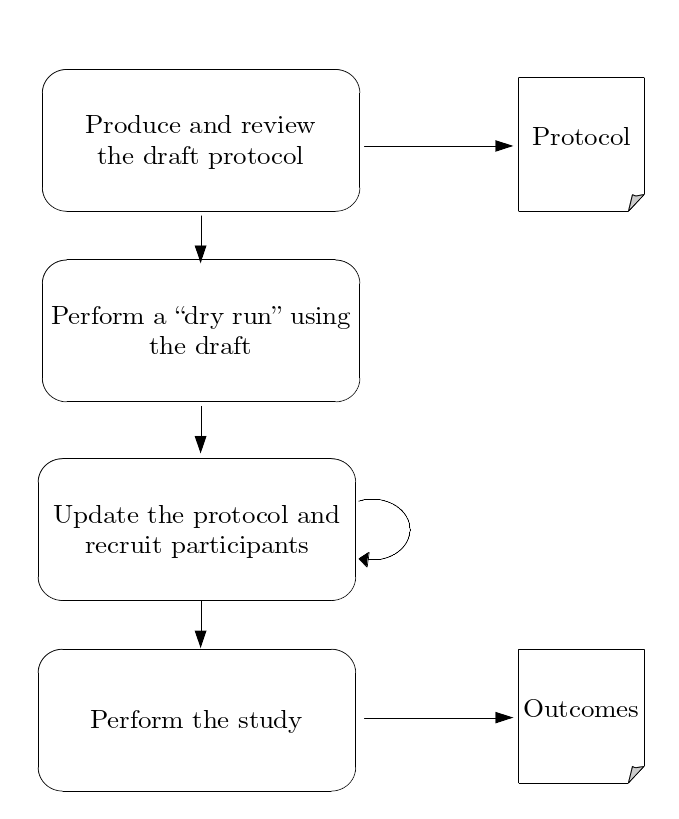
\includegraphics[scale=0.5]{dryrun}
\section{Primary studies in SE}
Major forms of primary studies used in software engineering research:
\begin{itemize}
	\item Controlled experiments
	\item Quasi experiments
	\item Surveys
	\item Case studies
\end{itemize}
\section{Randomised controlled trial (RCT)}
The ideal RCT includes:
\begin{itemize}
	\item Participants being unaware of whether they are receiving the treatment or a placebo (blinding)
	\item Those running the trial being unaware of who is receiving the treatment (double blinding)
	\item The analyst working out the result not knowing who was in the trial group (triple blinding)
\end{itemize}
In SE the only element we can blind is analysis
\subsection{Between subjects}
Participants are divided into two groups:
\begin{itemize}
	\item The "control", a group who performs their task using "standard" forms
	\item The "experimental group", who perform their task using the treatment under investigation
\end{itemize}
\section{Quasi-Experiments}
\begin{itemize}
	\item Quasi-experimental forms are used when it is impossible or impractical to perform random allocation of participants to a group
	\item Often used when participants are required to have specific skills or knowledge
	\item There are many ways to organise a quasi-experiment, including
	\begin{itemize}
		\item Cross-over forms
		\item Before-after forms
		\item Time interval forms
	\end{itemize}
\end{itemize}
\section{Analysis}
\begin{itemize}
	\item There will always be variation in the measured outcomes because we are using people and hence other factors may have an influence upon the outcomes
	\item This means that deciding between the hypothesis and the null hypothesis becomes a statistical task. By convention, aim for a 95\% confidence level
	\item Experimenters are expected to report the confidence level when they state their results
\end{itemize}
\section{Surveys}
Used to collect information from a large group of people in a standard and systematic way, so that we can seek patterns in the data and generalise what these imply for a wider population than our sample\\
\\
Typically used for two purposes:
\begin{itemize}
	\item \textbf{Experimental}: To assess the impact of some intervention
	\item \textbf{Descriptive}: So that we can make assertions about some phenomenon of interest and where we are less interested in why this occurs as to how much it does
\end{itemize}
\subsection{Key concepts}
We seek a sample of respondents who are suitably representative of a larger sample frame\\
\\
Selection is made through use of a sampling technique, this can be:
\begin{itemize}
	\item \textbf{Probabilistic} - random, systematic, stratified, cluster
	\item \textbf{Non-probabilistic} - self selection, snowballing, convenience
\end{itemize}
\subsection{Data collection}
\textbf{Questionnaires} provide consistency of data collection but
\begin{itemize}
	\item Limited as to type of question can use
	\item Response rates may be poor
\end{itemize}
\textbf{Interviews} can be either structured or semi-structured\\
\\
\textbf{Observations} requiring no direct involvement with the participants\\
\\
\textbf{Literature} perhaps using data mining
\subsection{Problems}
\begin{itemize}
	\item We rarely know the size of our sampling frame
	\item Difficult to identify and access a sample of participants
	\item Small sample sizes make it difficult to get results with a high confidence level
	\item It iq quite challenging to design questions that are unbiased and that allow users to answer them reliably
	\item In a well designed survey the questions will reinforce each other so that during analysis we can ensure that participants are giving consistent answers
\end{itemize}
\section{Case studies}
\begin{definition}[Case study]
A controlled form of observational field study, involving planned data collection
\end{definition}
A case study typically involves:
\begin{itemize}
	\item More variables of interest than data points
	\item Use of triangulation between multiple sources of evidence
	\item Prior development of propositions
\end{itemize}
\subsection{Types of case study}
\begin{definition}[Explanatory study]
Used to answer questions about how some phenomenon works and why it works
\end{definition}
\begin{definition}[Descriptive study]
Used to produce a rich and detailed analysis of a phenomenon and its context. Involves less detail about mechanisms than an explanatory study
\end{definition}
\begin{definition}[Exploratory study]
Used to lay the groundwork for a later fuller study, perhaps by helping identify the questions or help understand a problem
\end{definition}
\subsection{Use in software engineering}
Particularly useful when investigating how software engineering practices are adopted or used in an industry setting, where we have:
\begin{itemize}
	\item Limited control of the situation, so can only observe
	\item Relatively few "cases"
	\item Many diverse sources of data, project lots, minutes of meetings, interviews with the team
	\item A need to study an effect "in the field"
\end{itemize}

\end{document}